\documentclass[11pt]{article}
\usepackage[utf8]{inputenc}
\usepackage[T1]{fontenc}
\usepackage{graphicx}
\usepackage{longtable}
\usepackage{float}
\usepackage{wrapfig}
\usepackage{soul}
\usepackage{amssymb}
\usepackage{hyperref}
\usepackage[spanish]{babel}
\usepackage{bookman}
\usepackage[left=3cm,top=3cm,right=2cm,bottom=1cm,head=1.5cm,includefoot]{geometry}
\usepackage{listings}
\usepackage{multirow}
\usepackage{amssymb}
\usepackage{fancyhdr}
\usepackage{comment}
\usepackage{color}
\usepackage{multicol}
\usepackage[table]{xcolor}
\usepackage{ulem}

\title{informe}
\author{}

\begin{document}


\definecolor{gray97}{gray}{.97}
\definecolor{gray75}{gray}{.75}
\definecolor{gray45}{gray}{.45}

\lstset{linewidth=\textwidth}
\lstset{ frame=Ltb,
     framerule=0pt,
     aboveskip=0.5cm,
     framextopmargin=3pt,
     framexbottommargin=3pt,
     framexleftmargin=0.4cm,
     framesep=0pt,
     rulesep=.4pt,
     backgroundcolor=\color{gray97},
     rulesepcolor=\color{black},
     %
     stringstyle=\ttfamily,
     showstringspaces = false,
     basicstyle=\small\ttfamily,
     commentstyle=\color{gray45},
     keywordstyle=\bfseries,
     %
     numbers=left,
     numbersep=15pt,
     numberstyle=\tiny,
     numberfirstline = false,
     breaklines=true,
}


\pagestyle{fancy}
\lhead{
\includegraphics[width=1.5cm]{Logo-fiuba} }
\chead{75.59 - T\'ecnicas de Programaci\'on Concurrente I}
\rhead{\Huge FIUBA}
\lfoot{Trabajo Pr\'actico 2 }
\rfoot{$2^{do}$ cuatrimestre 2011}
\tableofcontents
\newpage


\section{Enunciado}

\begin{center}
% Orden del trim = izq abajo derecha arriba
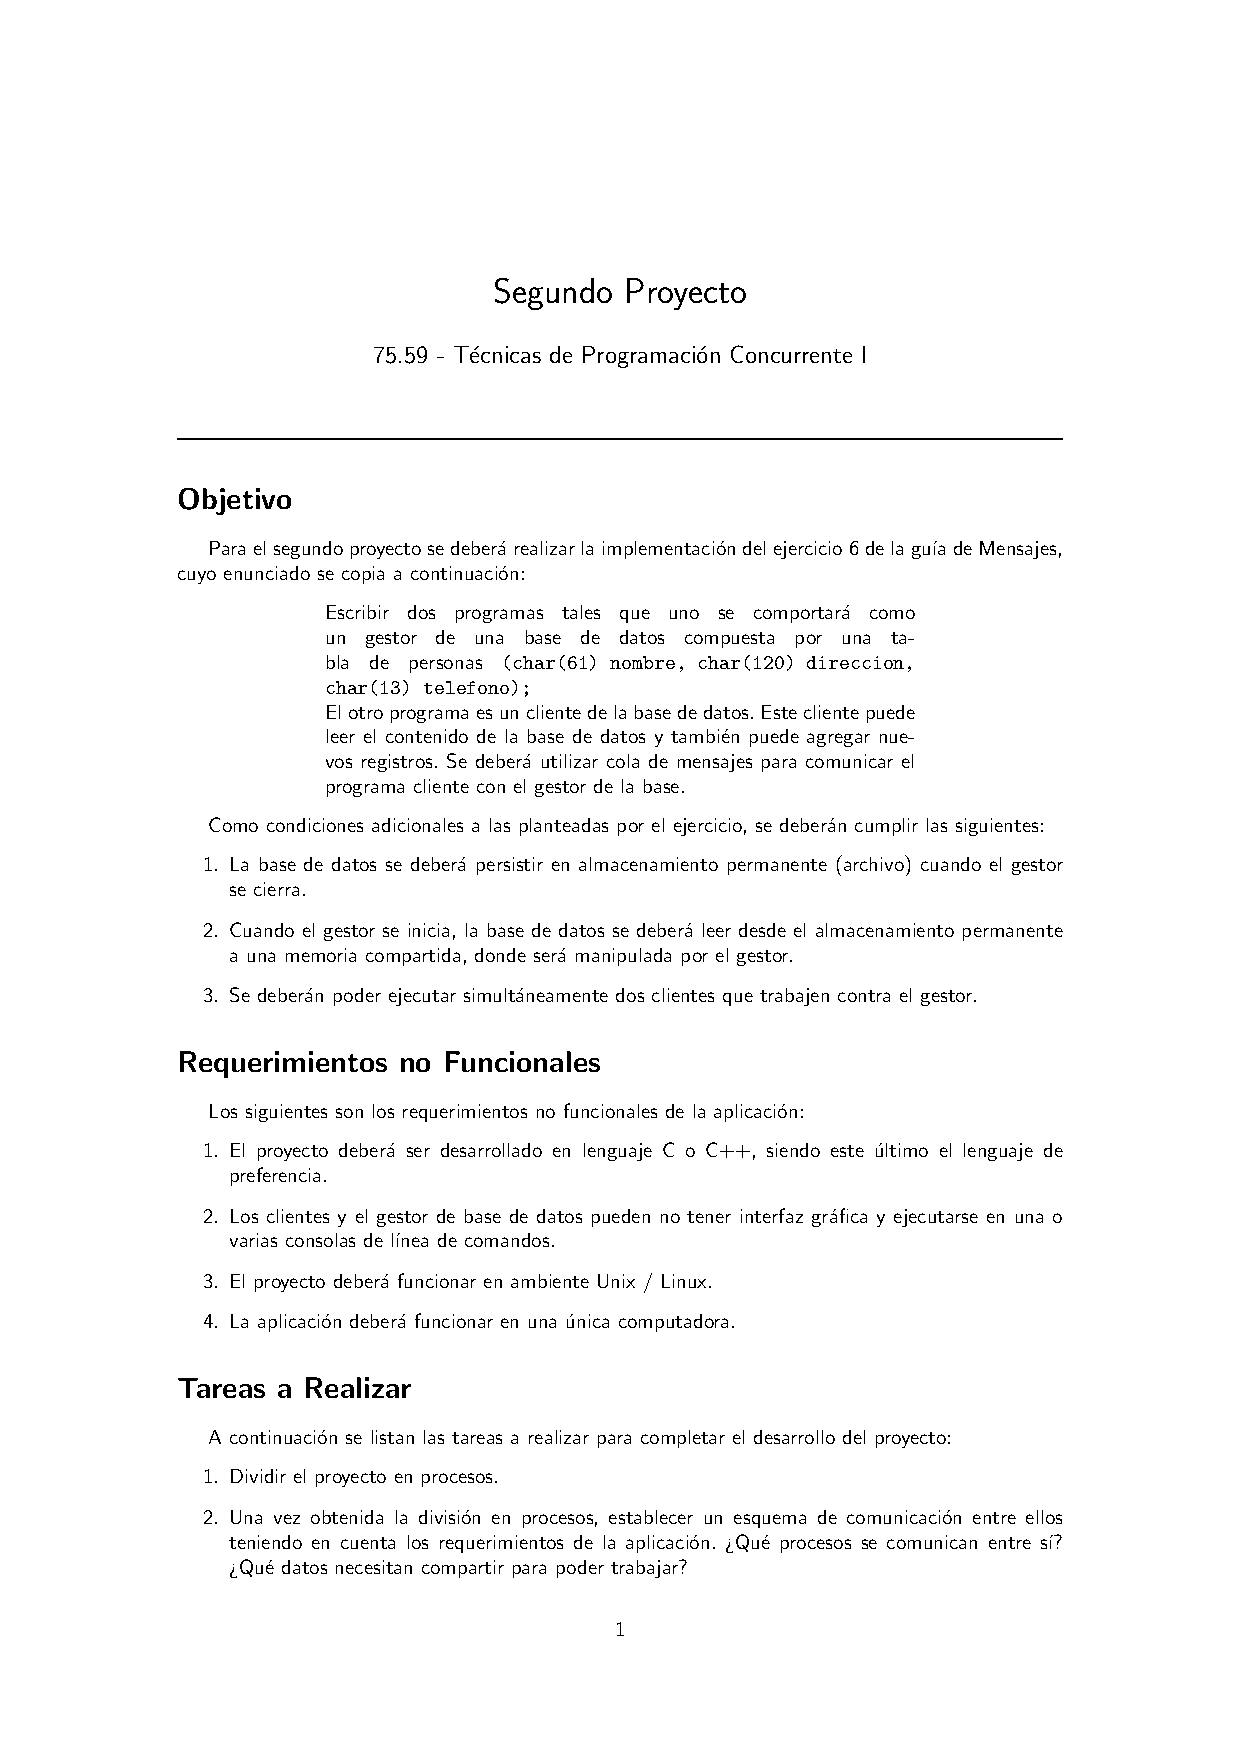
\includegraphics[trim = 25mm 30mm 10mm 35mm, clip,height=0.93\textheight,width=1.04\textwidth]{SegundoProyecto.pdf}
\includegraphics[trim = 25mm 20mm 10mm 30mm, clip,height=0.95\textheight,width=1.04\textwidth,page={2}]{SegundoProyecto.pdf}
\end{center}

\newpage


\section{Requerimientos Funcionales}

El sistema desarrollado permite realizar el alta, baja y modificaci\'on de los datos de una persona en la base de datos.
El mismo cuenta con dos aplicaciones diferentes; una corresponde al cliente y otra al gestor de la base de datos.


\section{Hip\'otesis}
\begin{itemize}
 \item Se utiliz\'o como clave primaria de la base de datos el campo nombre de cada registro. Es por este motivo, que se supone que si dos 
personas se llaman de igual forma, son la misma persona.
 \item Se supone que el gestor siempre va a tener lugar disponible en la cola de mensajes, para enviar la respuesta a una petición de algún cliente;
ya que en esta versión solo se ejecutan simultáneamente dos clientes.
\end{itemize}
\item 

\section{Consideraciones de Dise\~no}

\begin{itemize}
\item Se decidió desarrollar las aplicaciones en lenguaje C++, para utilizar el encapsulamiento de las clases.
\item Cada cliente se ejecuta en una consola distinta, al igual que el gestor.
\item Los campos permiten el ingreso de cadenas separadas por espacios, de forma tal de considerar los nombres compuestos, el ingreso de apellido y 
nombre de las personas, entre otras cosas.
\item Para el acceso a la memoria compartida se utiliz\'o un sem\'aforo, de forma tal de lograr sincronizar el mismo. Este sem\'aforo es \'unico 
para la base de datos en su totalidad.
\item Para acceder al archivo utilizado en la persistencia de la base de datos se utiliza un lockfile 
\item Al modificar una persona desde la aplicaci\'on cliente se le solicita al usuario que ingrese primero el nombre de la misma tal cual figura en la base de datos, 
y luego se le solicita que ingrese la nueva direcci\'on y tel\'efono. 
\item Antes de realizar alguna modificación en la base de datos, se pide la confirmación del usuario, para evitar registrar datos erróneos.
\end{itemize}


\section {Comunicaci\'on entre procesos}

Para realizar la comunicaci\'on entre los procesos gestor y cliente se utiliz\'o una \textit{Cola de Mensajes}, dado que la misma permite comunicarlos 
aunque no posean relaci\'on entre ellos, siendo en este caso dos aplicaciones diferentes. La ventaja que posee la 
cola de mensajes es que la misma permite enviar estructuras de datos completas a trav\'es de ella; en lugar de bytes como en los fifos.
Esto implica que no sea necesario sincronizar la escritura de varios procesos en la misma, dado que no puede suspenderse la escritura 
de dicha estructura antes de finalizar la misma. Es decir, no puede darse el caso de que por cambiar el ipc, el uso de cpu a otro proceso escriba uno la mitad de su estructura 
en la cola y el otro comience desde allí.
Al mismo tiempo, la utilizaci\'on de colas de mensajes simplifica el protocolo de comunicaci\'on entre los procesos, dado que es posible utilizar los campos de la estructura 
como por ejemplo, el dato long obligatorio para identificar que proceso es destinatario de cada uno de los mensajes. Esto último posibilita que la cola de mensajes sea bidireccional.

La estructura utilizada para transmitir los mensajes a trav\'es de la cola es la siguiente:

\begin{lstlisting}[language=C]
 typedef struct {
	long mtype;
	pid_t id;
	T_PETICION tipo;
	Registro registro;
	char respuesta[256];
} mensaje;
\end{lstlisting}

A continuaci\'on se presenta una descripci\'on de cada uno de los campos que conforman dicha estructura.
\begin{itemize}
\item mtype: es un long obligatorio que se utiliza para indicar el destinatario del mensaje.
\item id: es el n\'umero de proceso de quien env\'ia el mensaje.
\item tipo: es un enumerado que representa el tipo de petici\'on del mensaje en cuesti\'on. 
Los valores posibles para este campo son los siguientes: ``AGREGAR, ELIMINAR, CONSULTAR, MODIFICAR''
\item registro: es una estructura que contiene las cadenas de caracteres con los datos de la persona que se desea agregar, modificar, eliminar o sobre la que 
se desea consultar.
\item respuesta: es una cadena de caracteres que se utiliza para enviar mensajes desde el gestor hacia los clientes, 
informandoles el resultado de la operaci\'on realizada.
\end{itemize}


\subsection{Protocolo utilizado}
El protocolo de comunicaci\'on utilizado se desprende de observar la estructura anterior. A continuaci\'on se describe el formato 
de los mensajes que se transmiten mediante la cola, de forma tal de aclarar cada uno de los tipos de mensajes utilizados para establecer la 
comunicaci\'on entre los procesos. \\
Para los mensajes que parten desde los clientes hacia el gestor se conforman de la siguiente manera:
\begin{itemize}
 \item mtype = PETICION
 \item id = pid\_del\_proceso\_que\_envia
 \item tipo = AGREGAR \'o ELIMINAR \'o CONSULTAR \'o MODIFICAR
 \item registro = Datos\_de\_la\_persona\_requeridos\_por\_la\_operacion
 \item respuesta = `` ''
\end{itemize}


Para los mensajes que parten desde el gestor hacia los clientes se conforman de la siguiente manera:
\begin{itemize}
 \item mtype = pid\_del\_cliente\_que\_debe\_recibirlo
 \item id = `` ''
 \item tipo = `` ''
 \item registro = Datos\_consultados\_de\_la\_persona
 \item respuesta = mensaje\_informando\_el\_resultado\_de\_la\_operaci\'on
\end{itemize}

El gestor lee los mensajes que tengan como mtype el valor PETICION y los clientes leen los mensajes cuyo mtype corresponda al id de su proceso.
De esta manera la cola de mensajes es bidireccional y cada cliente va a obtener la respuesta que le corresponda, ya que el pid es único para cada proceso.

\section{Herramientas de concurrencia utilizadas}
\begin{itemize}

 \item \underline{Cola de mensajes}: utilizada para resolver la comunicaci\'on entre los procesos cliente y gestor. \\
 \item \underline{Memoria compartida}: utilizada para almacenar la base de datos. Permitir\'ia, en caso de existir mas de un gestor, que todos los gestores 
compartan la informaci\'on all\'i almacenada.  \\
 \item \underline{Sem\'aforo}: utilizado para obtener sincronismo en el acceso a la memoria compartida que contiene la base de datos. \\
 \item \underline{LockFiles}: utilizado para sincronizar la persistencia de la base de datos en un archivo, de forma tal de garantizar que solo un
gestor acceda a este recurso a la vez, en caso de existir mas de uno. \\
 \item \underline{Se\~nales}: utilizada para detener la ejecuci\'on del proceso gestor que esta esperando una petición. Se utiliza la se\~nal SIGINT en este caso para finalizar de forma correcta el gestor de base de datos. \\
\end{itemize}



\section{Casos de Uso}

%\subsection{Cliente}

\begin{center}
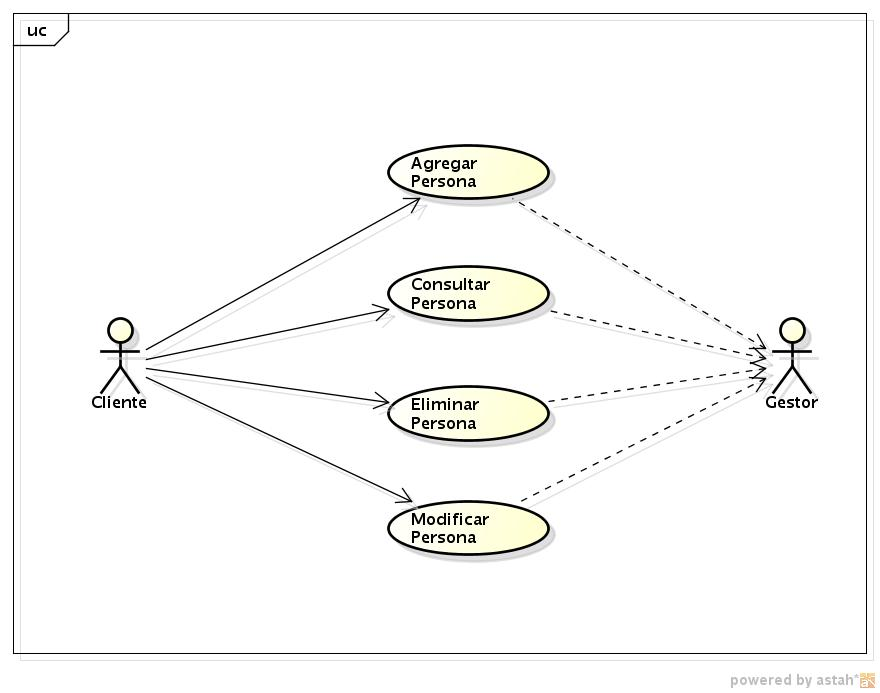
\includegraphics[scale=0.65]{CasosUsoCliente} 
\end{center}

%\subsubsection{Especificaci\'on de los casos de uso del Cliente}
\subsubsection{Especificaci\'on de los casos de uso}
  \begin{tabular}{|l|m{0.8\textwidth}|}
    \hline
    \multicolumn{2}{|m{0.9\textwidth}|}{{\bf Caso de uso: Agregar Persona}} \\
    \hline
    \multicolumn{2}{|l|}{\rowcolor[gray]{.5}} \\
    \hline
  
    \multicolumn{2}{|p{0.9\textwidth}|}{{\bf Descripción:} Alta de los datos de una 
    persona en la base de datos } \\
  
    \hline
    \multicolumn{2}{|l|}{Actores participantes: Cliente} \\
    \hline
  
    \multicolumn{2}{|l|}{Pre-condiciones: Se deben haber ejecutado las aplicaciones cliente 
    y gestor} \\
  
    \hline
    \multicolumn{2}{|l|}{\rowcolor[gray]{.5}} \\
    \hline
    \multicolumn{2}{|l|}{Flujo Principal} \\
    \hline
    1 & El actor cliente ingresa a la aplicaci\'on. \\
    \hline
    2 &  El actor indica la acción a realizar \newline
    Si la acción es el alta de una nueva persona entonces ejecutar subflujo Alta de persona (S1)\newline
   \\
    
    \hline
    \multicolumn{2}{|l|}{Flujos Alternativos} \\
    \hline
  
    S1 &  Alta de persona: \\ \hline
    S1.1 & El sistema solicita el ingreso del nombre de la persona a dar de alta.\\ \hline
    S1.2 & El cliente ingresa el nombre de la persona\\ \hline
    S1.3 & El sistema valida que el nombre de dicha persona no exista ya en la base de datos (E1) \\ \hline
    S1.4 & El sistema solicita el ingreso de la direcci\'on de dicha persona\\ \hline
    S1.5 & El cliente ingresa la direcci\'on de la persona\\ \hline
    S1.6 & El sistema solicita el ingreso del tel\'efono de dicha persona\\ \hline
    S1.7 & El sistema procesa el registro, arma la petici\'on y se la env\'ia al gestor.\\ \hline
    S1.8 & El caso de uso comienza nuevamente desde el paso 2.\\ \hline
    
    \multicolumn{2}{|l|}{Flujos de Excepción} \\
    \hline
  
    E1 & Ya existe una persona con dicho nombre, se le informa al cliente y se vuelve al men\'u anterior. 
    El caso de uso finaliza.\\
  
    \hline
    \multicolumn{2}{|l|}{\rowcolor[gray]{.5}} \\
    \hline
  
    \multicolumn{2}{|m{0.9\textwidth}|}{Post-condiciones: Se agregaron los datos de la nueva persona a la base de datos
    y desde este momento est\'a disponible dicha informaci\'on para el resto de los clientes} \\
  
    \hline
  \end{tabular}
  \newline

\begin{tabular}{|l|m{0.8\textwidth}|}
    \hline
    \multicolumn{2}{|m{0.9\textwidth}|}{{\bf Caso de uso: Modificar Persona}} \\
    \hline
    \multicolumn{2}{|l|}{\rowcolor[gray]{.5}} \\
    \hline
  
    \multicolumn{2}{|p{0.9\textwidth}|}{{\bf Descripción:} Modificaci\'on de los datos de una 
    persona en la base de datos } \\
  
    \hline
    \multicolumn{2}{|l|}{Actores participantes: Cliente} \\
    \hline
  
    \multicolumn{2}{|l|}{Pre-condiciones: Se deben haber ejecutado las aplicaciones cliente 
    y gestor} \\
  
    \hline
    \multicolumn{2}{|l|}{\rowcolor[gray]{.5}} \\
    \hline
    \multicolumn{2}{|l|}{Flujo Principal} \\
    \hline
    1 & El actor cliente ingresa a la aplicaci\'on. \\
    \hline
    2 &  El actor indica la acción a realizar \newline
    Si la acción es la modificaci\'on de los datos de una persona entonces ejecutar subflujo Modificaci\'on de persona (S1)\newline
   \\
    
    \hline
    \multicolumn{2}{|l|}{Flujos Alternativos} \\
    \hline
  
    S1 &  Modificaci\'on de persona: \\ \hline
    S1.1 & El sistema solicita el ingreso del nombre de la persona a modificar.\\ \hline
    S1.2 & El cliente ingresa el nombre de la persona\\ \hline
    S1.3 & El sistema valida que el nombre de dicha persona ya exista en la base de datos (E1) \\ \hline
    S1.4 & El sistema solicita el ingreso de la direcci\'on de dicha persona\\ \hline
    S1.5 & El cliente ingresa la direcci\'on de la persona\\ \hline
    S1.6 & El sistema solicita el ingreso del tel\'efono de dicha persona\\ \hline
    S1.7 & El sistema procesa el registro, arma la petici\'on y se la env\'ia al gestor.\\ \hline
    S1.8 & El caso de uso comienza nuevamente desde el paso 2.\\ \hline
    
    \multicolumn{2}{|l|}{Flujos de Excepción} \\
    \hline
  
    E1 & Si no existe una persona con dicho nombre, se le informa al cliente y se vuelve al men\'u anterior. 
    El caso de uso finaliza.\\
  
    \hline
    \multicolumn{2}{|l|}{\rowcolor[gray]{.5}} \\
    \hline
  
    \multicolumn{2}{|m{0.9\textwidth}|}{Post-condiciones: Se modificaron los datos de la persona en la base de datos} \\
  
    \hline
  \end{tabular}
  \newline

\begin{tabular}{|l|m{0.8\textwidth}|}
    \hline
    \multicolumn{2}{|m{0.9\textwidth}|}{{\bf Caso de uso: Eliminar Persona}} \\
    \hline
    \multicolumn{2}{|l|}{\rowcolor[gray]{.5}} \\
    \hline
  
    \multicolumn{2}{|p{0.9\textwidth}|}{{\bf Descripción:} Baja de los datos de una 
    persona en la base de datos } \\
  
    \hline
    \multicolumn{2}{|l|}{Actores participantes: Cliente} \\
    \hline
  
    \multicolumn{2}{|l|}{Pre-condiciones: Se deben haber ejecutado las aplicaciones cliente 
    y gestor} \\
  
    \hline
    \multicolumn{2}{|l|}{\rowcolor[gray]{.5}} \\
    \hline
    \multicolumn{2}{|l|}{Flujo Principal} \\
    \hline
    1 & El actor cliente ingresa a la aplicaci\'on. \\
    \hline
    2 &  El actor indica la acción a realizar \newline
    Si la acción es la baja de una persona entonces ejecutar subflujo Baja de persona (S1)\newline
   \\
    
    \hline
    \multicolumn{2}{|l|}{Flujos Alternativos} \\
    \hline
  
    S1 &  Baja de persona: \\ \hline
    S1.1 & El sistema solicita el ingreso del nombre de la persona a dar de baja.\\ \hline
    S1.2 & El cliente ingresa el nombre de la persona\\ \hline
    S1.3 & El sistema valida que el nombre de dicha persona exista en la base de datos (E1) \\ \hline
    S1.4 & El caso de uso comienza nuevamente desde el paso 2.\\ \hline
    
    \multicolumn{2}{|l|}{Flujos de Excepción} \\
    \hline
  
    E1 & No existe una persona con dicho nombre, se le informa al cliente y se vuelve al men\'u anterior. 
    El caso de uso finaliza.\\
  
    \hline
    \multicolumn{2}{|l|}{\rowcolor[gray]{.5}} \\
    \hline
  
   \multicolumn{2}{|m{0.9\textwidth}|}{Post-condiciones: Se eliminaron los datos de la persona en la base de datos} \\
  
    \hline
  \end{tabular}
  \newline

\begin{tabular}{|l|m{0.8\textwidth}|}
    \hline
    \multicolumn{2}{|m{0.9\textwidth}|}{{\bf Caso de uso: Consultar Persona}} \\
    \hline
    \multicolumn{2}{|l|}{\rowcolor[gray]{.5}} \\
    \hline
  
    \multicolumn{2}{|p{0.9\textwidth}|}{{\bf Descripción:} Consulta de los datos de una 
    persona en la base de datos } \\
  
    \hline
    \multicolumn{2}{|l|}{Actores participantes: Cliente} \\
    \hline
  
    \multicolumn{2}{|l|}{Pre-condiciones: Se deben haber ejecutado las aplicaciones cliente 
    y gestor} \\
  
    \hline
    \multicolumn{2}{|l|}{\rowcolor[gray]{.5}} \\
    \hline
    \multicolumn{2}{|l|}{Flujo Principal} \\
    \hline
    1 & El actor cliente ingresa a la aplicaci\'on. \\
    \hline
    2 &  El actor indica la acción a realizar \newline
    Si la acción es la consulta de los datos de una persona entonces ejecutar subflujo Consulta de persona (S1)\newline
   \\
    
    \hline
    \multicolumn{2}{|l|}{Flujos Alternativos} \\
    \hline
  
    S1 &  Consulta de persona: \\ \hline
    S1.1 & El sistema solicita el ingreso del nombre de la persona a consultar.\\ \hline
    S1.2 & El cliente ingresa el nombre de la persona\\ \hline
    S1.3 & El sistema valida que el nombre de dicha persona exista en la base de datos (E1) \\ \hline
    S1.4 & El sistema procesa la petici\'on\\ \hline
    S1.5 & El sistema informa nombre, direcci\'on y tel\'efono de la persona consultada\\ \hline
    S1.6 & El caso de uso comienza nuevamente desde el paso 2.\\ \hline
    
    \multicolumn{2}{|l|}{Flujos de Excepción} \\
    \hline
  
    E1 & No existe una persona con dicho nombre, se le informa al cliente y se vuelve al men\'u anterior. 
    El caso de uso finaliza.\\
  
    \hline
    \multicolumn{2}{|l|}{\rowcolor[gray]{.5}} \\
    \hline
  
    \multicolumn{2}{|m{0.9\textwidth}|}{Post-condiciones: Se obtuvieron los datos de la persona consultada de la base de datos} \\
  
    \hline
  \end{tabular}
  \newline


%\subsection{Gestor}

%\begin{center}
%\includegraphics[scale=0.65]{CasosUsoGestor} 
%\end{center}

%\subsubsection{Especificaci\'on de los casos de uso del Gestor}





\newpage

\section{Diagrama de clases}
 En esta secci\'on se presentan los diagramas de clase para cada una de las aplicaciones.
\subsection{Diagrama de clases Cliente}
A continuaci\'on se observa el diagrama de clases correspondiente a la aplicaci\'on cliente. Es importante aclarar que se incluye la clase Mensaje, 
siendo en realidad una estructura. Esta última se muestra en el diagrama dado que la clase Cola es de tipo template, y en este caso, es utilizada 
con dicha estructura. 
\begin{center}
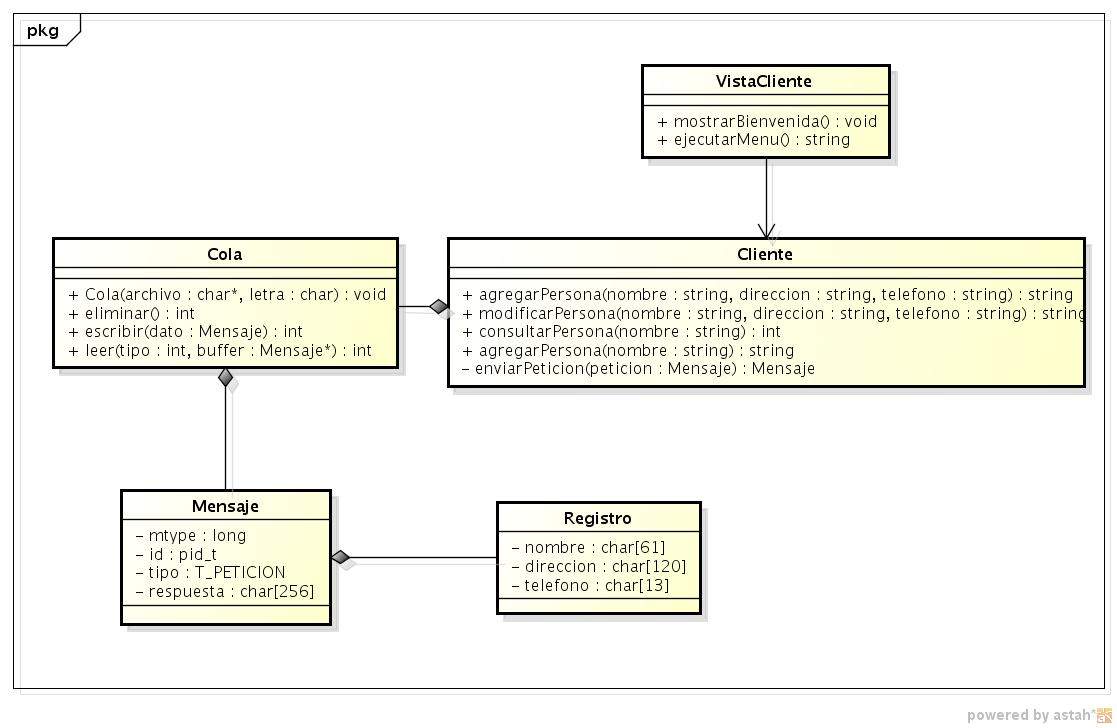
\includegraphics[scale=0.45,width=1.02\textwidth]{ClasesCliente} 
\end{center}


\subsection{Diagrama de clases Gestor}
A continuaci\'on se observa el diagrama de clases para la aplicaci\'on gestor. Se incluye la clase Mensaje por las mismas razones enunciadas anteriormente.
Para simplificar la apreciaci\'on del diagrama se decidi\'o no mostrar en el mismo los m\'etodos y atributos privados de las clases en cuest\'on.

\begin{center}
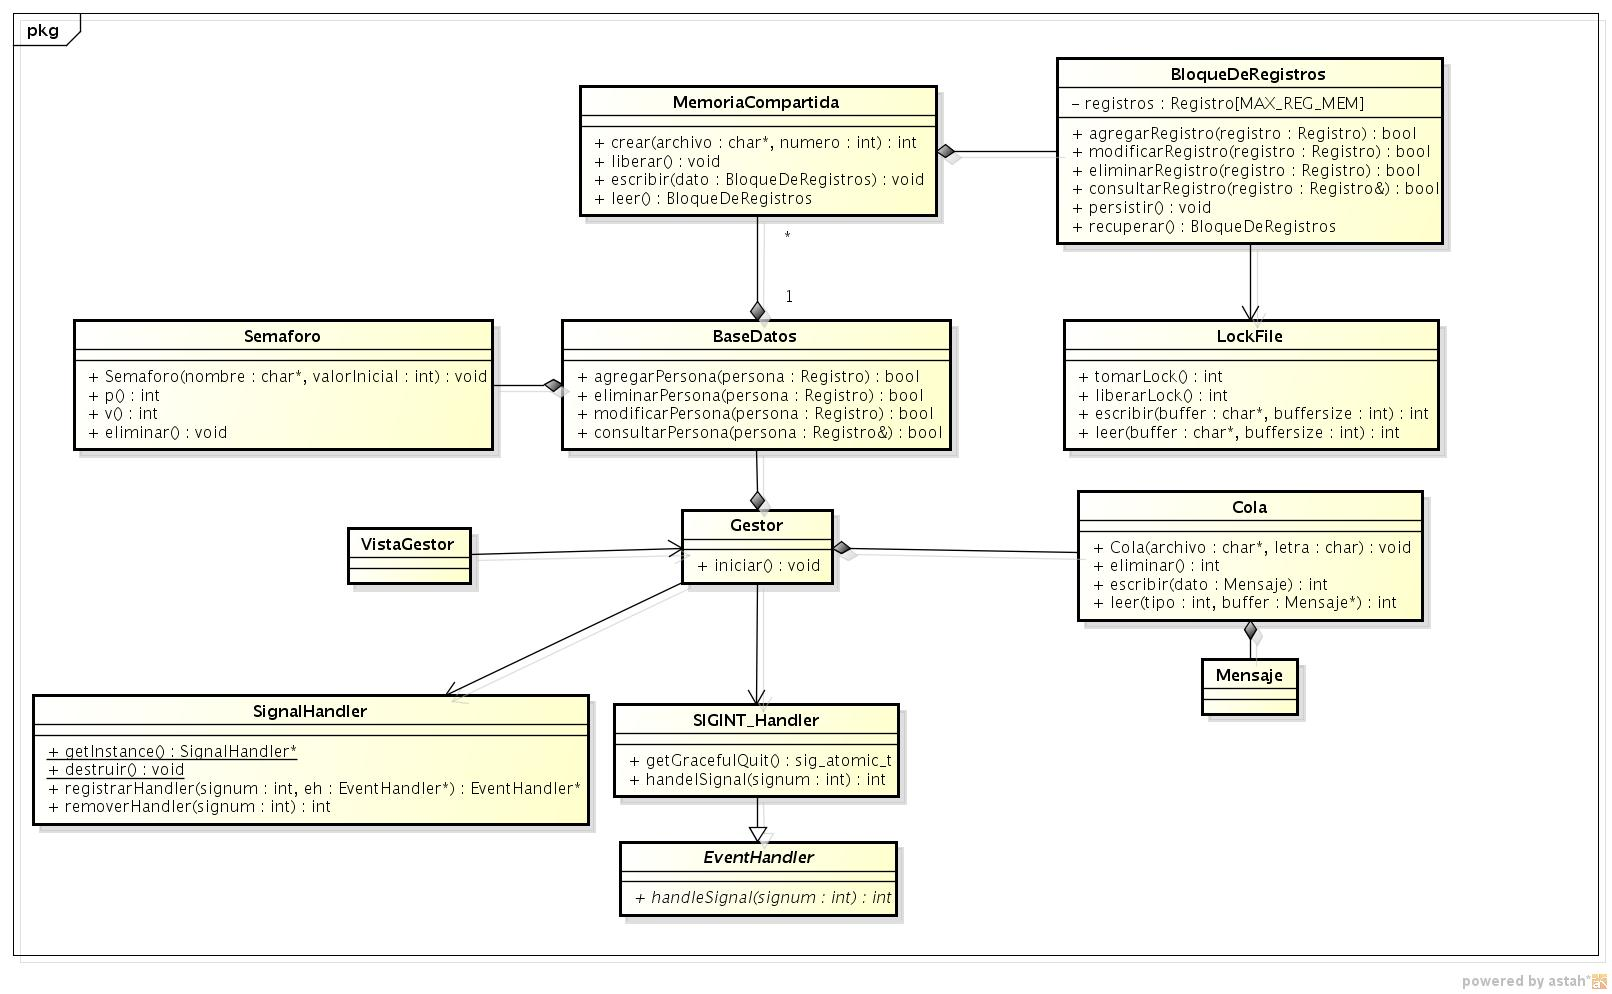
\includegraphics[scale=0.45, height=0.93\textheight,width=1.02\textwidth]{ClasesGestor} 
\end{center}

\newpage
\section{Compilaci\'on}
Con el fin de facilitar la compilaci\'on de las aplicaciones se provee un script bajo el nombre {\bf compilar.sh}. El mismo se encuentra ubicado en 
el directorio en el cu\'al se encuentra el c\'odigo fuente, y se utiliza de la siguiente forma:
\begin{itemize}
 \item Ubicarse en el directorio en el cu\'al se encuentra el c\'odigo fuente de las aplicaciones. Para ello puede utilizarse el siguiente 
comando desde un ambiente Unix\/Linux:\\
\$~:cd Directorio\_del\_trabajo\_practico
\item Ejecutar el siguiente comando: \\
\$~:./compilar.sh
\subitem * El script {\bf compilar.sh} debe contar con permisos de ejecuci\'on para poder realizar la compilaci\'on.
\item Una vez finalizada la compilaci\'on del paso anterior, se observar\'an, en dicho directorio, dos archivos ejecutables: \textit{cliente} y \textit{gestor}. 
Estos archivos representan respectivamente a las aplicaciones cliente y gestor, y para ejecutarlos debe utilizarse {\bf ./cliente} y {\bf ./gestor}. 
\end{itemize}


\section{Modo de Uso}
Para utilizar la aplicaci\'on {\bf gestor} debe considerarse que la misma finaliza al presionar la tecla \textit{'s'} en la consola en la cu\'al esta corriendo; 
esto es informado en la misma mediante un mensaje. \\ \\
Para utilizar la aplicaci\'on {\bf cliente} se debe respetar la interfaz por consola que la misma presenta. \\

\newpage


\section{Conclusiones}



\end{document}

